\documentclass[11pt,a4paper]{article}
\newcommand{\manualname}{RackNES}
\newcommand{\manualversion}{2.2.0}
\usepackage{kautenjadsp-manual}
\begin{document}
\manualcover{RackNES}{A voltage-controlled Nintendo Entertainment System}
\manualchapter{Overview and first sound}{sec:quick-start}
RackNES runs an NES game inside VCV Rack 2. The game supplies the music,
sound effects, and visuals; your patch controls the players, changes the
emulation speed, and returns to saved moments. Five separate sound outputs
and a mix output connect the game to the rest of your rack.

The module starts without a game. Supply an iNES ROM file and use the panel
buttons or gates as the two NES controllers. A game's response to those
buttons depends on its menus and current play state.

\subsection{Start here}
\begin{enumerate}
\item Add RackNES and connect \textbf{MIX} to your audio output through a
mixer or attenuator. Begin with a low listening level.
\item Leave all five channel levels and Mix Volume at their default
\textbf{100\%}. Leave the large clock knob at its default
\textbf{1.789773 MHz} and the red clock attenuverter at \textbf{0\%}.
\item Right-click RackNES, choose \textbf{Load ROM}, and select a
\texttt{.nes} or \texttt{.NES} file. You can also drop one ROM file onto the
module. The supported cartridge mappers are listed on page~\pageref{sec:roms}.
\item Use Player 1 \textbf{Start}, \textbf{Select}, the directions, and
\textbf{A/B} to reach a part of the game that makes sound. Hold a panel
button for as long as the game requires.
\item Press \textbf{SAVE} at an interesting moment. Let the game continue,
then press \textbf{LOAD} to revisit it. There is one snapshot slot.
\end{enumerate}

\subsection{Three useful first experiments}
\begin{description}
\item[Separate the percussion.] Patch \textbf{NOI} to a second mixer input.
Noise disappears from MIX and can now have its own effects chain.
\item[Automate a controller.] Send a repeating gate to Player 1 A.
A high gate holds the button; a low gate releases it.
\item[Repeat a game moment.] Send a slow trigger to LOAD after making a
snapshot. Each trigger restores the stored emulation state.
\end{description}

\subsection{What to expect}
RackNES is an emulator under voltage control. Its clock input changes the
speed of execution; it does not receive tempo pulses for synchronization.
SAVE and LOAD store machine state, not an audio clip. Hang freezes execution
and holds the outputs. The following sections explain these distinctions
and the limitations of the current implementation.

\manualchapter{Panel guide}{sec:panel}
\begin{center}
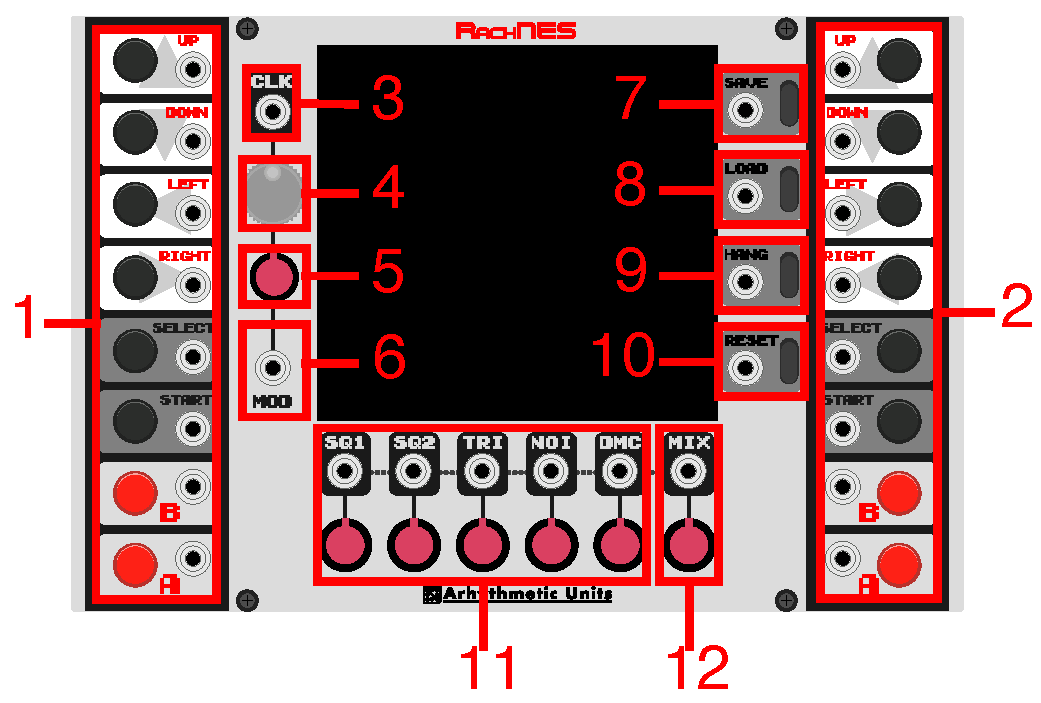
\includegraphics[width=\textwidth]{img/RackNES-Manual}
\end{center}
\begin{tabularx}{\textwidth}{@{}r l X@{}}
\toprule
\textbf{No.} & \textbf{Control} & \textbf{Use} \\
\midrule
1--2 & Players 1 and 2 & Hold buttons by hand or with gates (p.~\pageref{sec:controllers}). \\
3 & CLK output & Frame-counter clock at 0/10 V (p.~\pageref{sec:clock}). \\
4 & Clock Speed & Set the emulation rate. \\
5 & Clock attenuverter & Set the amount and polarity of speed CV. \\
6 & MOD input & Add CV to the speed setting. \\
7 & SAVE & Replace the stored snapshot (p.~\pageref{sec:state}). \\
8 & LOAD & Restore the stored snapshot. \\
9 & HANG & Hold execution while pressed or gated high. \\
10 & RESET & Reset the NES with the current ROM inserted. \\
11 & Voice outputs / levels & SQ1, SQ2, TRI, NOI, DMC (p.~\pageref{sec:audio}). \\
12 & MIX output / level & Sum voices whose separate jacks are unpatched. \\
\bottomrule
\end{tabularx}

The center screen shows the emulated video. It is a display, not a touch
controller. The illustrated light panel and the dark panel have the same
controls and routing.

\manualchapter{ROMs and compatibility}{sec:roms}
\subsection{Loading a game}
Choose \textbf{Load ROM} from the module's right-click menu, or drag a ROM
file onto the panel. The chooser accepts \texttt{.nes} and \texttt{.NES}.
Extract compressed archives first.

Loading a ROM, including the same ROM again, resets the emulator and clears
SAVE. Canceling leaves the current selection alone. Only the first dropped
file is used.

\subsection{Supported cartridge mappers}
A mapper arranges cartridge memory. RackNES supports these six IDs;
individual games and modified ROMs may still behave incorrectly.
\begin{center}
\begin{tabular}{@{}rl@{\hspace{3em}}rl@{}}
\toprule
\textbf{ID} & \textbf{Name} & \textbf{ID} & \textbf{Name} \\
\midrule
0 & NROM & 3 & CNROM \\
1 & MMC1 & 7 & AxROM / AOROM \\
2 & UNROM & 9 & MMC2 / PxROM \\
\bottomrule
\end{tabular}
\end{center}
Mapper 7 accepts 32--256 KiB of PRG ROM in power-of-two sizes, 8 KiB of
CHR RAM, and either one-screen nametable page. Legacy iNES and NES 2.0
submappers 0/1 use no bus conflicts; submapper 2 combines writes with the
visible PRG byte. Only NTSC layouts are accepted. CHR ROM, battery RAM,
trainers, four-screen layouts, extra devices, and other variants are rejected.
Legacy headers cannot reliably identify every board variant.

Mapper 9 accepts power-of-two PRG ROM sizes of 32--128 KiB, CHR ROM sizes
of 8--128 KiB, and 8 KiB PRG RAM, with optional battery metadata. Supported
formats are NTSC iNES and NES 2.0 submapper 0. Trainers, CHR RAM, four-screen
layouts and other variants are rejected. RAM persists in Rack patches and
SAVE snapshots; external battery-save files are not imported or exported.

Timing is fixed; there is no PAL/NTSC or mapper selector. Audio uses the five
base NES voices without cartridge expansion sound. CV Genie's game list
contains memory maps and does not define ROM compatibility.

\subsection{When loading fails}
\begin{description}
\item[ASIC mapper not implemented for ROM!]
The file requests a mapper outside the implemented set, or an unsupported
mapper-7 or mapper-9 image layout.
\item[ROM file failed to load!]
The selected path failed ROM validation. Check the file and its format.
\item[ROM file was not found!]
A patch's stored ROM path could not be validated on restore. Check that the
same ROM is still present at that path.
\end{description}
A failed new-ROM attempt leaves the current game, display, and SAVE slot
in place. Correct the file selection and try again.

\textbf{Moving patches.} Keep the original ROM at its saved path: restoration
reloads that file. Loading a ROM manually starts a new session; it does not
recover a failed snapshot restore.

\manualchapter{Controllers and gate inputs}{sec:controllers}
Each player has eight momentary buttons and eight matching CV inputs:
\textbf{Up, Down, Left, Right, Select, Start, B, A} from top to bottom.
Player 1 is on the left edge and Player 2 on the right.

\subsection{Hold a button with a gate}
A controller button is pressed while either its panel button or its CV gate
is high. Release both to release the virtual button. A held gate is a held
button, not a stream of repeated presses. For repeated presses, use a pulse
train with a low interval between pulses.

Both players are available simultaneously. The game decides whether Player 2
is active, and what simultaneous or opposing directions mean. RackNES does
not turn these inputs into keyboard or physical gamepad mappings.

\subsection{Thresholds and timing}
The controller, SAVE, LOAD, HANG, and RESET CV inputs use hysteresis:
a rising signal reaches the high state at about \textbf{2 V}, and must
return to about \textbf{0.1 V} or below to re-arm. The intermediate region
retains the previous state. Ordinary 0--5 V or 0--10 V gates are suitable.

These inputs are checked once every \textbf{16 Rack samples}. At 48 kHz,
that is approximately 0.333 ms. Very short pulses can fall between checks.
For controller actions, hold a gate long enough for the game itself to read
it; a pulse that RackNES detects may still be too short for a game's input
polling. Try tens of milliseconds or longer when a game misses a press.

All inputs read the first channel of a cable. Polyphonic voices do not act
as separate controllers or combine into a larger gate.

\subsection{Triggers and held controls}
\begin{tabularx}{\textwidth}{@{}p{.26\textwidth}X@{}}
\toprule
\textbf{Control} & \textbf{Response} \\
\midrule
Player buttons & Pressed for the duration of the high state. \\
SAVE / LOAD / RESET & Act once on a rising edge. A sustained high gate does not repeat the action. \\
HANG & Suspends execution for the duration of the high state. \\
\bottomrule
\end{tabularx}

Panel buttons and CV triggers are detected separately. For example, pressing
LOAD by hand can restore a snapshot even while its CV input is already
high. Controller and Hang states instead use the combined held state.

\manualchapter{Clock speed and clock output}{sec:clock}
\subsection{Change the rate of the game}
The large knob sets a requested CPU rate around \textbf{1.789773 MHz}.
Its range is one sixteenth to sixteen times that rate, approximately
\textbf{0.111861--28.636368 MHz}. It changes how quickly the game runs and
issues sound commands. It is not a calibrated musical pitch control.

The red attenuverter starts at \textbf{0\%}, so MOD has no effect until you
turn it. Positive settings let positive voltage speed up execution;
negative settings reverse the effect. At +100\%, adding 5 V doubles the
requested rate and subtracting 5 V halves it, until the limits are reached.

\begin{center}
\begin{tabular}{@{}rrl@{}}
\toprule
\textbf{MOD voltage} & \textbf{Attenuverter} & \textbf{Rate relative to knob} \\
\midrule
+5 V & +100\% & $2\times$ \\
+10 V & +100\% & $4\times$ \\
+5 V & $-100\%$ & $1/2\times$ \\
Any & 0\% & Unchanged \\
\bottomrule
\end{tabular}
\end{center}
These are requested ratios before clamping and sample-step rounding. The
knob's MHz readout describes its base setting; it does not include MOD.
Use a slow CV first. High speed settings increase the amount of emulation
work per Rack sample.

\subsection{Use CLK as a clock source}
CLK is a \textbf{0 V / 10 V} square wave with approximately 50\% duty cycle.
It follows a counter of \textbf{29,781 emulated CPU cycles}, approximately
one frame. It is not the raw MHz CPU clock and is not synchronized to a
specific musical beat in a game. With no running game the counter does not
advance; the output may stay high instead of producing pulses.

A divider after CLK can supply slower events to sequencers or percussion.
Changing Clock Speed changes this output too. MOD accepts a speed voltage,
so sending a clock pulse into MOD alternates between two speeds; it does
not lock RackNES to that pulse train.

\subsection{Timing and sound limits}
The implementation executes a whole number of CPU cycles on each Rack
sample, rounding the requested cycle count upward. At 48 kHz and the default
knob setting, it executes 38 cycles per sample and CLK is about
\textbf{61.25 Hz}. The ideal requested ratio alone would suggest about
60.10 Hz. Rack sample rate therefore affects the realized clock.

Audio buffering uses a separate fixed conversion clock in this version.
Clock Speed should be treated as an experimental game-speed control;
neither clean tape-style transposition nor exact pitch tracking is promised.
Hang holds CLK at its current voltage, and LOAD does not reset its counter
phase. See page~\pageref{sec:reference} for the exact control equation.

\manualchapter{Save, load, hang, and reset}{sec:state}
\subsection{SAVE: keep one moment}
Press SAVE or send a rising trigger to replace the one stored emulator
snapshot. It includes game and machine state, not a recorded audio waveform.
The slot belongs to this instance of RackNES. A later SAVE overwrites it.

\subsection{LOAD: return to the stored moment}
Press LOAD or send a rising trigger to restore the slot. Without a saved
snapshot, LOAD does nothing. Repeat LOAD to revisit a sound effect, phrase,
or gameplay event. Panel knob positions and patch cables are not part of
this slot, so you can change the mix or speed while reusing a game moment.

Snapshots are not sample-accurate audio loops. The frame-counter phase and
queued audio samples are not serialized with the machine state. Controller
inputs also continue to update, so different gates after a restore can lead
the game in a different direction. Discontinuities at a load can click;
shape an external VCA if you need smoother transitions.

\subsection{HANG: hold execution}
Hold HANG or its input gate high to suspend CPU, video, and audio advancement.
The module returns before refreshing its output jacks, so audio and CLK
\textbf{hold their last voltages}; Hang does not mute them to zero and does
not sustain a synthesized note normally. The screen stops advancing too.

Control acquisition and CV Genie messages still run while hung. You can
SAVE, LOAD, or RESET, and an attached Genie can still write memory. Release
both the panel button and the CV gate to resume execution and output updates.

\subsection{RESET: restart the inserted game}
The panel RESET button and its input reset the CPU, video, and audio systems
with the current ROM inserted. They leave the SAVE slot available. This is
a console reset, not a promise that all game RAM becomes a fresh power-on
image.

Rack's module \textbf{Initialize} action is different: its reset handler
removes the ROM, clears the snapshot, and blanks the screen. Loading a ROM
from the context menu also clears the snapshot when successful.

\subsection{Simultaneous actions and patch saving}
If SAVE, RESET, and LOAD rise in the same control update, RackNES processes
them in that order. SAVE captures the pre-reset state and LOAD restores it.
This avoids replacing the saved moment with the just-reset one.

Saving the Rack patch includes the current emulator state and the SAVE slot
if one exists. Keep the ROM at its original path for both to restore.
A saved patch is the way to retain your session; there is no separate
snapshot-file import/export menu.

\manualchapter{Voices and mixing}{sec:audio}
The five voice outputs follow the NES audio channels. What each contains
changes as the game plays music and sound effects.
\begin{center}
\begin{tabularx}{\textwidth}{@{}l X@{}}
\toprule
\textbf{Jack} & \textbf{Voice} \\
\midrule
SQ1 / SQ2 & Two pulse (square) voices, often used for melody and harmony. \\
TRI & Triangle voice, often used for bass. \\
NOI & Noise voice, often used for percussion and sound effects. \\
DMC & Delta-modulated sample voice. It can be silent in games or passages that do not use it. \\
MIX & Sum of the voices whose individual outputs are unpatched. \\
\bottomrule
\end{tabularx}
\end{center}

\subsection{Separate outputs remove voices from MIX}
Patch a voice's jack to take it out of MIX. Its level knob still controls
its individual output. Unplug the jack to return it to MIX. This routing
change depends on the cable connection, even if the receiving module is
muted. Connecting all five voice outputs leaves MIX with no voices.

Each voice level runs from \textbf{0\% to 200\%}, starting at 100\%.
It affects that voice before either the separate jack or MIX. Mix Volume
also runs from 0\% to 200\% and only scales MIX; it has no effect on the
separate outputs.

\subsection{Levels are content-dependent}
The audio conversion maps a full-scale signed sample to approximately
$\pm10$ V before the voice gain. This does \textbf{not} guarantee a 10 V
peak-to-peak waveform at each jack. Actual amplitude depends on the NES
voice and the game. At 200\%, the voice gain doubles its voltage.

MIX adds the unpatched voices and applies its own gain; it is not normalized
to their number and has no output limiter. Lower levels in RackNES or use
an external mixer when combining voices. A downstream device can clip even
when RackNES's own controls remain in range.

\subsection{Try it: process just the noise}
Keep MIX connected to one mixer channel. Connect NOI to a filter or delay,
then to another mixer channel. Noise now takes the effects path while the
other voices stay in MIX. Use the NOI knob to set the effects send level,
and the external mixer to balance the two paths.

Audio outputs are monophonic. Separate voices are separate jacks, not
polyphonic channels in the MIX cable.

\manualchapter{Patch ideas}{sec:patches}
\subsection{Repeat a phrase with LOAD}
\begin{enumerate}
\item Load a game, start its music, and press SAVE just before an event.
\item Send a slow, regular trigger to LOAD. Each rising edge revisits that
moment; adjust the interval to choose how far the game advances.
\item Try different channel levels or route voices to separate effects.
\item Move SAVE to a new moment when you want to replace the phrase.
\end{enumerate}
An independent Rack clock is useful here. CLK's phase is not restored by
LOAD, so it is not a sample-accurate loop marker.

\subsection{Make the game control the patch}
Patch CLK to a clock divider, then use the divided outputs to trigger
percussion or advance a sequencer. Turn Clock Speed slowly to move both
the game and the downstream events. The correspondence is to the emulator's
frame counter, not to the game's internal music tempo.

\subsection{Play with gates}
Send separate gate patterns to Player 1 A and a direction. Use longer gates
for movement and shorter, separated gates for repeated button presses.
Try SAVE/LOAD to revisit the same starting situation while comparing
patterns. The result depends on the game's input handling.

\subsection{Alternate between two speeds}
With the main clock knob near its center, send a 0--5 V gate to MOD and turn
the attenuverter toward +100\%. The requested rate doubles during the high
part of the gate. Reduce the attenuverter for gentler changes, or make it
negative to slow the game during each gate.

\subsection{Add CV Genie}
Place \textbf{CV Genie (Input)} immediately to the right of RackNES. Select
the matching game and assign the memory locations you want to control.
Unassigned rows remain inactive, even with CV connected. Genie can alter game data such as position, palette, or the
Zelda sound-driver state. Its separate manual lists the maps and the
important setup limitations. RackNES accepts only the directly adjacent
input Genie; a chain of Genies does not extend the eight inputs.

\manualchapter{Control values and settings}{sec:reference}
\begin{tabularx}{\textwidth}{@{}p{.30\textwidth}p{.25\textwidth}X@{}}
\toprule
\textbf{Control} & \textbf{Range} & \textbf{Initial setting} \\
\midrule
Clock Speed & $1/16$--$16\times$ base & 1.789773 MHz \\
Speed CV attenuverter & $-100\%$ to $+100\%$ & 0\% (CV off) \\
Voice levels (five) & 0--200\% & 100\% each \\
Mix Volume & 0--200\% & 100\% \\
Controller / action buttons & Momentary & Released \\
ROM / SAVE slot & One of each & Empty \\
CLK output & 0 or 10 V & Static until counter advances \\
\bottomrule
\end{tabularx}

\subsection{Clock equation}
Let $k$ be the knob's internal setting ($-4$ to $+4$), $a$ the attenuverter
($-1$ to $+1$), and $v$ the MOD voltage in volts. The requested rate is
\[
f_{\mathrm{request}}=1{,}789{,}773\;2^{\operatorname{clamp}(k+av/5,-4,4)}
\quad\text{cycles/s}.
\]
The implementation converts this to an integer rate, then performs
\[
N=\left\lceil\frac{\lfloor f_{\mathrm{request}}\rfloor}{f_s}\right\rceil
\quad\text{cycles per Rack sample},\qquad
f_{\mathrm{CLK}}\approx\frac{Nf_s}{29{,}781},
\]
where $f_s$ is Rack's sample rate. Floating-point rounding can affect exact
boundary cases. These equations describe execution and CLK, not a promised
pitch ratio for the audio outputs. CLK stops cycling when execution stops.

\subsection{Light and dark panels}
Right-click either module and choose \textbf{Light} or \textbf{Dark} under
the \textbf{Plugin Theme} heading. Selecting a theme
changes that instance's panel immediately and stores the plugin-wide default
in \texttt{RackNES.json} in Rack's user folder. Newly created widgets use
that default. Other already-open instances do not all switch immediately.
The choice is a user preference, not a per-patch theme setting.

\subsection{Persistence at a glance}
Rack saves panel parameters and cabling with the patch. RackNES adds current
emulator state and the optional SAVE slot. Theme is stored separately.
The ROM file must remain accessible, and restoring a snapshot does not
restore an exact audio-buffer or clock phase.

\manualchapter{Troubleshooting and further reading}{sec:troubleshooting}
\begin{description}
\item[No picture or no game response.]
Load a supported ROM and release HANG and its gate. Check for a load-error
dialog. A title screen may need Start or Select before the game responds.
\item[The screen moves but there is no sound.]
Reach a part of the game that makes sound. Check the voice levels and Mix
Volume. Voices with patched individual outputs are removed from MIX.
If all five are patched, MIX is silent. Check your downstream audio routing.
\item[A gate does nothing or works only once.]
Reach about 2 V to activate, then return below about 0.1 V to re-arm.
Lengthen very short pulses. Controller actions also depend on game polling;
a held gate is a held button.
\item[Clock CV has no effect.]
The attenuverter starts at zero. Turn it up and keep the base knob away
from its limits. MOD takes a speed voltage, not a synchronization clock.
\item[LOAD does nothing or the loop is inconsistent.]
Make a snapshot first. Loading a new ROM or initializing the module clears
it. Gate patterns and game logic can change what happens after LOAD, and
snapshots do not contain the audio queue or frame-clock phase.
\item[HANG leaves a voltage on the audio or clock jack.]
This is the implemented behavior. Use an external VCA or mute if you need
silence while the machine is held.
\item[The saved patch cannot find its game.]
Restore the same ROM to the stored path and reopen the patch. Loading a
ROM manually starts a fresh session and clears the snapshot slot.
\item[High-speed operation is expensive or sounds rough.]
Reduce Clock Speed and its modulation depth. The implementation does more
CPU emulation work per Rack sample at high rates; its audio conversion does
not guarantee smooth resampling across speed changes.
\end{description}

\subsection{Sources and acknowledgments}
This manual follows the module controls, emulator, audio wrapper, and theme
handling in the repository's \texttt{src/} directory. The maintainer's
\href{https://github.com/Kautenja/RackNES/tree/master/manual}{manual guide}
maps each topic to its implementation.
RackNES builds on Amish Naidu and contributors' SimpleNES; Shay Green's
(blargg's) Nes\_Snd\_Emu, Blip\_Buffer, and nes\_ntsc; and Ren\'e
Nyffenegger's cpp-base64. The
\href{https://github.com/Kautenja/RackNES/blob/master/LICENSING.md}{license guide}
links the bundled component notices and license texts. CV Genie was developed
by \textbf{@anlexmatos}. The companion
\href{https://github.com/Kautenja/RackNES/releases/latest/download/CVGenie.pdf}{CV Genie manual}
covers its eight input rows and memory maps.

\manualcolophon
\end{document}
